\chapter{Balance de carga en SPS}
\label{cap:estadoDelArte}

\section{Perspectivas de balance de carga}
\label{sec:perspectivasBC}
Dentro de la literatura se ha observado distintas perspectivas del problema de balance de carga en un SPS, las cuales consideran los recursos f\'isicos como fuente del problema, o los recursos l\'ogicos como el foco del mismo.

\subsection{Recursos f\'isicos}
\label{subsec:recFisicosBC}
En esta perspectiva se toma en consideraci\'on la sobrecarga del sistema dado las limitantes f\'isicas de \'este, ya sea por condiciones de los recursos disponibles o por el ambiente de desarrollo. Las estrategias de balance de carga que se presentan est\'an basados en el concepto de umbrales de recursos, es decir, \normalsize{cuando estos} umbrales son alcanzados se aplica una estrategia para aliviar la carga. Estos umbrales pueden ser el nivel \textit{Service Level Objective} (SLO) \citep{sturm2000foundations}, porcentaje de CPU utilizada o disponibilidad de la memoria \citep{dong2006scheduling}, entre otros.

Una de las soluciones con la perspectiva anterior es Borealis \citep{XingZH05}. Borealis considera la cantidad de carga de los nodos en ventanas de tiempo pre-determinadas, las cuales son monitoreadas por un coordinador centralizado. Este coordinador se encarga de analizar los recursos del sistema, y en caso que se sobrepase el umbral propuesto, se aplica la migraci\'on de los operadores del nodo hacia a otro nodo candidato cuya carga es menor.

%Esta estrategia no soluciona el problema de rendimiento del sistema, debido a que s\'olo mueve el problema de una m\'aquina a otra. Para elegir al nodo candidato, se realiza un an\'alisis de correlaci\'on que existe entre el operador y el nodo candidato, de esta manera, no necesariamente va a ser enviado a otro nodo con menor carga, sino tambi\'en al m\'as cercano. Dentro de los problemas que pueden existir en este sistema radican la conexi\'on entre los distintos nodos, por lo que para las pruebas se considera un buen ancho de banda de tal manera que aparente una red sin limitaciones de este tipo.

Si bien esta estrategia realiza una balance de carga en cuanto a las m\'aquinas f\'isicas, no aumenta el rendimiento dado los recursos l\'ogicos disponibles, dado que s\'olo mueve el operador sobrecargado de una m\'aquina a otra. En el trabajo anterior, para elegir el nodo candidato se realiza una an\'alisis de correlaci\'on existente entre el operador y el nodo candidato, de tal manera de no s\'olo enviarlo al nodo con menor carga, sino el que entre menor latencia en la interacci\'on con el operador. Uno de los problemas existes en este sistema radican en la conexi\'on entre los distintos nodos, por lo que para las pruebas se ha considerado un alto ancho de banda, de tal manera que aparente una red sin limitaciones de este tipo.

Por otra parte, Flood \citep{Alves2010flood} propone un DPS (\textit{Distributed data stream processing}) que considera factores f\'isicos para agregar o eliminar m\'aquinas virtuales en Amazon EC2 \citep{amazonec2}. Para esto, se utiliza un administrador que considera las estad\'isticas en tiempo de ejecuci\'on como la cantidad de CPU utilizada, latencia o memoria disponible. Estas estad\'isticas permiten ver en que rango de carga se encuentra la m\'aquina seg\'un los umbrales establecidos, para posteriormente agregar o eliminar m\'aquinas.

\subsection{Recursos l\'ogicos}
\label{subsec:recLogicosBC}
%A diferencia de la f\'isica, aqu\'i se consideran los componentes l\'ogicos del sistema, como por ejemplo, una sobrecarga en alg\'un operador. De esta manera, en las distintas soluciones se pueden encontrar soluciones en cuanto a la carga existente en el operador o la cantidad de cola que posea, de tal manera, que estos sean los umbrales a considerar para generar una mejora en el sistema.

A diferencia de la perspectiva basada en recursos f\'isicos, en esta perspectiva se consideran los componentes l\'ogicos del sistema, es decir, el foco est\'a en los operadores y su carga de trabajo. Las distintas soluciones que se presentan bajo esta mirada, analizan componentes como el flujo de datos o el tama\~no de la cola de un operador, tom\'andolos como par\'ametros y definiendo umbrales en los algoritmos implementados para determinar cuando realizar las mejoras al sistema.

% Enfoques de la perspectiva l\'ogica

Existen dos tipos de enfoques: est\'atico y din\'amico \citep{Gupta99loadsharing}. El primer enfoque est\'a centrado en un modelo predefinido y que se mantiene fijo luego de la inicializaci\'on del sistema, sin considerar el estado del mismo. \normalsize{\'Este se caracteriza por una implementaci\'on de bajo costo computacional, comparado con el enfoque din\'amico, el cual es utilizado en general por los SPS. Por otra parte, el segundo enfoque est\'a basado en un modelo el cual analiza el sistema seg\'un su estado en tiempo de ejecuci\'on, donde se utilizan pol\'iticas para optimizar el rendimiento de \'este.}

%El primer enfoque se centra en la confecci\'on de un modelo definido y fijo antes de iniciar el sistema y que no var\'ia en el tiempo. En cambio, el segundo se basa en la adaptaci\'on del sistema seg\'un su estado en tiempo de ejecuci\'on.

\subsection{Enfoque est\'atico}
\label{subsec:enfoqueEstaticoBC}
Este enfoque se ha implementando en distintos sistemas de procesamiento de \textsl{stream} y consiste en definir previo a la ejecuci\'on, la cantidad de operadores para la aplicaci\'on. De esta manera, no existe una interrupci\'on en la ejecuci\'on o un cambio luego de la ejecuci\'on. \citep{CasavantK88}.

%\textsl{Storm} utiliza la t\'ecnica de distribuci\'on de operadores seg\'un alguna pol\'itica, tomando el enfoque est\'atico \citep{stormtwitter}. El sistema configura el n\'umero de operadores que son necesarios para realizar una tarea, para que despu\'es estos sean repartidos en los distintos nodos disponibles seg\'un la pol\'itica de \textit{Shuffle grouping}. Esta t\'ecnica basada en algoritmos de planificaci\'on \citep{bookScheduling}, consiste en distribuir los operadores en los distintos nodos utilizando una planificaci\'on \textsl{Round-Robin}, de tal manera que la cantidad de operadores sea uniforme en los nodos del sistema \citep{bookstorm}.

\textsl{Storm} utiliza distintas t\'ecnicas de distribuci\'on de las tuplas en los operadores seg\'un la pol\'itica que se desee, todas tomando un enfoque est\'atico \citep{stormtwitter}. Dentro de las pol\'iticas que existen est\'an \textit{Shuffle grouping}, \textit{Fields grouping}, \textit{Partial Key grouping}, \textit{All grouping}, \textit{Global grouping}, \textit{None grouping}, \textit{Direct grouping} y \textit{Local grouping}.

La pol\'itica de \textit{Shuffle grouping} se enfoca en distribuir las tuplas de forma homog\'eneas en los $n$ operadores que se encuentren en el grafo utilizando la planificaci\'on \textit{Round-Robin} \citep{bookScheduling}. De esta manera la cantidad de tuplas se distribuye de forma homog\'enea en el sistema. Una de las principales fallas es que la tasa de procesamiento de las tuplas no siempre es la misma, por lo tanto puede existir una sobrecarga en un operador en particular, dado que \'este recibe tuplas que requieren un mayor tiempo de procesamiento.

\textit{Fields grouping} determina ciertas llaves a un operador determinado. Por ejemplo, se contiene un flujo de datos que se identifican por el nombre de los usuarios, de ser as\'i, desde cierto rango de letras corresponden a cierto operador, de tal manera de dividir equitativamente seg\'un la cantidad de caracteres existentes. Si bien genera un determinismo en el procesamiento de las llaves, puede existir una sobrecarga de un operador en particular, debido a que una llave se puede repetir con mayor frecuencia que otras, lo cual es demostrado en la ley de potencia \citep{rushton2010handbook}.

%Otra t\'ecnica es el uso de la funci\'on \textsl{hash} \citep{RogawayS04} para distribuir los operadores en el grafo, como lo planteado en S4 \citep{s4yahoo}. Esto consiste en aplicar lo anterior a alg\'un atributo del evento, mapeando el evento al operador que corresponda de los $n$ operadores disponibles seg\'un el valor de la funci\'on. Cabe destacar que si no existe un operador mapeado con la imagen de la funci\'on, el sistema clona uno existente evaluando el nuevo con la imagen de la funci\'on como identificador. De esta manera, esta t\'ecnica provee dinamicidad respecto a la cantidad de operadores en el sistema.

Por otra parte, se encuentra el funcionamiento de S4, cuya pol\'itica es similar a la de \textit{Fields grouping} de Storm. La diferencia es que un operador no le corresponde un conjunto de llaves, sino que posee una llave \'unica. Esto quiere decir que cada llave se le asigna un operador, y en caso de no existir un operador para el valor de esa llave, se crea un nuevo operador de manera autom\'atica. Debido a la infinidad de combinaciones de llaves que pueden generarse, S4 recomienda aplicar una funci\'on \textit{consistent hashing} para evitar posibles colisiones \citep{X11cp}. Esta t\'ecnica provee dinamismo en la cantidad de operadores en el sistema, pero al igual que la \textit{Fields grouping} puede sobrecargar un operador, debido que una llave puede poseer mayor frecuencia que las otras, como se expresa en la ley de potencia, debido que un porcentaje de llaves es m\'as usada que otras, como es el caso de las palabras utilizadas en el diccionario \citep{rushton2010handbook}.

Una ventaja del enfoque est\'atico es el bajo costo de la implementaci\'on de los m\'etodos, comparado con modelos matem\'aticos o modelos planteados por el enfoque din\'amico, lo cual es beneficioso para sistemas con escasos recursos y con restricciones de tiempo de respuesta. Por otra parte, una desventaja considerable es la existencia de puntos cr\'iticos en la topolog\'ia, es decir, que un operador recibe m\'as carga que sus pares, por lo que no se asegura que la cantidad de flujo sea repartido de forma homog\'enea. Si bien, no es una soluci\'on \'optima, es un buen complemento para un modelo con el enfoque din\'amico.

\subsection{Enfoque din\'amico}
\label{subsec:enfoqueDinamicoBC}

%Este enfoque est\'a basado en el estado del sistema, donde seg\'un las variables y estado de cada uno de sus atributos, genera una acci\'on en el sistema \citep{CasavantK88}. Esto significa que si el sistema posee alguna anomal\'ia, como una sobrecarga en un operador o latencia entre distintos nodos, se realiza un cambio en el sistema, con el fin de solucionar estos problemas. Para poder dar una soluci\'on al problema de sobrecarga, se pueden utilizar dos tipos de modelos: reactivo y predictivo.

Este enfoque est\'a basado en el estado del sistema en ejecuci\'on, siendo esto el par\'ametro base para optimizar su rendimiento \citep{CasavantK88}. Esto significa que si el sistema posee un operador sobrecargado, se realiza un cambio en la l\'ogica del sistema con el fin de solucionar el problema. En este contexto se consideran dos modelos: reactivo y predictivo.

\paragraph{Reactivo:} este modelo est\'a basado en el an\'alisis de carga en a trav\'es de un monitor \citep{GulisanoJPSV12}, el cual recibe peri\'odicamente la informaci\'on de carga de cada uno de los operadores, y en caso que sobrepase un umbral, se aplica una t\'ecnica para balancear la carga y con ello aumentar el rendimiento. El umbral puede estar basado en el tiempo de procesamiento, el tama\~no de la cola u otra variable del operador \citep{BhuvanagiriGKS06}. Por ejemplo, en el trabajo de Schneider \citep{SchneiderAGBW09} se considera el rendimiento de cada operador. En caso de existir congesti\'on en el operador, se procede a replicarlo de tal manera que exista un operador adicional que puede recibir un flujo de datos y realizar en paralelo la misma operaci\'on que el operador sobrecargado.

%Si bien estas soluciones en su mayor\'ia son eficientes y poseen buen rendimiento, uno de los principales problemas es que no analiza el comportamiento a futuro, debido que s\'olo analiza y resuelve la situaci\'on en el momento. Otro problema son los falsos positivos, debido que puede ser que en un momento exista un \textit{peak} de tr\'afico, pero esto era s\'olo un caso particular del instante, por lo que llevar a cabo la replicaci\'on del operador es un costo innecesario.
Si bien estas soluciones en su mayor\'ia son eficientes, al otorgar un mejor rendimiento del sistema, uno de los principales problemas es que no analiza el comportamiento a futuro, debido que s\'olo analiza y resuelve la situaci\'on en el momento. \normalsize{Otro problema que puede surgir, corresponde a los falsos positivos, dado que puede existir un \textit{peak} en el tr\'afico en una ventana de tiempo peque\~na, pero eso no significa que ese comportamiento determine el flujo entrante.}

\paragraph{Predictivo:} este modelo est\'a basado en modelos matem\'aticos que calculan o estiman el comportamiento a futuro del sistema, utilizando informaci\'on hist\'orica relativa a flujo entrante, CPU u otra variable. Si bien no existen modelos predictivos para SPS, si los existen en otras \'areas, como se present\'o en la Secci\'on \ref{subSec:markovTrabajo} con cadenas de Markov y an\'alisis de series temporales en \textit{Cloud Computing}.

\section{T\'ecnicas de balance de carga}
\label{sec:tecnicasBC}

Existen distintas t\'ecnicas de balance de carga que utilizan alguno de los dos modelos presentados anteriormente, las cuales est\'an enfocadas a mejorar el rendimiento del sistema en caso de existir una sobrecarga \citep{HirzelSSGG13}. Dentro de las t\'ecnicas existentes se encuentran la planificaci\'on determinista \citep{XuCTS14, DongTS07}, \textit{load shedding} \citep{SheuC09}, migraci\'on \citep{XingZH05} y fisi\'on \citep{GulisanoJPSV12, IshiiS11, GedikSHW14, FernandezMKP13}, si bien existen m\'as, s\'olo se trataron estas porque se consideran las m\'as relevantes y que han sido trabajadas en la literatura relacionada al dominio del problema.

\subsection{Planificaci\'on determinista}
\label{sec:planificacionBC}
%La planificaci\'on determinista \citep{DongTS07} se centra en la planificaci\'on seg\'un los recursos y estados del sistema \textit{a priori} seg\'un alguna m\'etrica \citep{XuCTS14}. Una m\'etrica utilizada es la frecuencia de datos estimada en un nodo u operador \citep{Ganguly09}. Esta t\'ecnica se utiliza, por ejemplo, en \textit{StreamIt} \citep{ThiesKA02}. Una de las limitaciones es que si bien realiza una predicci\'on determinista de la frecuencia, no necesariamente es correcta a futuro, por lo que no se puede predecir las tasas de tr\'afico en el transcurso del procesamiento, sino s\'olo estimarlas al comienzo de la ejecuci\'on del sistema.

La planificaci\'on determinista se centra en los conocimientos \textit{a priori} del sistema. Esto significa que se consideran las variables del entorno que se poseen y respecto a esto se toma una decisi\'on de c\'omo debe actuar el sistema. 

En el \'area de \textit{Stream processing} se ha realizado diferentes an\'alisis de la estimaci\'on de frecuencia de \textit{data stream} en el sistema. Para esto, se ha considerado modelos matem\'aticos, tomando ventanas de tiempo de la frecuencia predicha y la real, para posteriormente generar con los datos una funci\'on que represente la frecuencia estimada del operador, es decir, el tr\'afico esperado que llega al operador en la ejecuci\'on del sistema \citep{Ganguly09}. \normalsize{Tambi\'en existen algoritmos} que determinan la frecuencia del sistema dado el flujo de datos que se puede recibir a futuro \citep{BhuvanagiriGKS06}.

En otras \'areas como red de sensores, se utiliza esta t\'ecnica en el env\'io de estad\'isticas de dispositivos m\'oviles, los cuales manejan informaci\'on \textit{a priori} de donde est\'an los sensores. De esta manera, se determina seg\'un la intensidad de la frecuencia, localizaci\'on o clima, a donde debe enviar la se\~nal para que se recolecte la informaci\'on deseada \citep{DongTS07}.

Una de las limitaciones de la t\'ecnica, es que si bien realiza una predicci\'on determinista de la frecuencia, no necesariamente es correcta a futuro. Esto se debe a que puede analizarse respecto al promedio, sin embargo pueden surgir \textit{peaks} o sucesos inesperados del tr\'afico en el transcurso de la ejecuci\'on que pueden generar una sobrecarga en el sistema. Por lo tanto, la estimaci\'on al realizarse \textit{a priori}, s\'olo considera los datos del inicio del sistema o los de ventanas de tiempo anteriores, por lo que puede existir un porcentaje de error considerable. Por otra parte, se considera que esta t\'ecnica posee mejor rendimiento si es que la frecuencia o funci\'on analizada es estacionaria o comportamientos repetitivos, pero no sucesos inesperados, como es el caso de las redes sociales, debido que suceden eventos externos que influyen en el tr\'afico analizado \citep{KarpSP03}.

% Darle una vuelta a esto...

%Es por esto, que no se considera una buena t\'ecnica para aplicar en los casos de estudio, debido que se desea trabajar con tr\'aficos din\'amicos, los cuales no poseen an\'alisis estacionarios, sino 

\subsection{Load Shedding}
\label{sec:loadSheddingBC}
%Otra estrategia est\'a orientada a descartar eventos de un operador sobrecargado, de tal manera de no generar colas en el sistema. Esta estrategia que si bien no est\'a implementada en el sistema por defecto de S4, puede habilitarse \citep{s4}. Otro ejemplo, es la trasmisi\'on de v\'ideo \textit{streaming}, donde se descartan los datos que son de baja calidad, para procesar en su mayor\'ia informaci\'on de alta calidad \citep{SheuC09}. Esta soluci\'on est\'a pensada para disminuir la carga, perdiendo la exactitud de la informaci\'on debido a la p\'erdida de datos. Por lo tanto existe una menor fiabilidad en el sistema en caso de realizar operaciones de transacci\'on \citep{bookDistrSys}.

En los SPS tambi\'en se utiliza la t\'ecnica de \textit{load shedding}, que consiste en descartar eventos del sistema en caso de existir operadores sobrecargados, ya sea \normalsize{en t\'erminos del} tama\~no de la cola, tasa de rendimiento u otro factor. En la Figura \ref{fig:loadShedding} se observa que existe un operador A, el cual recibe datos en un per\'iodo de tiempo, pero debido a la cola existente en el sistema, se considera utilizar un operador denominado \textit{Shedding}, que en caso de existir una cola mayor al umbral propuesto, \'este descarta los eventos candidatos seg\'un la m\'etrica establecida. Por ejemplo, en la transmisi\'on de \textit{video streaming}, al enviar el flujo de informaci\'on existe un administrador que est\'a analizando el contenido a procesar, por lo que en caso de llegar datos de baja calidad y existir cola, son descartados por \'este. De esta manera, al existir menor cantidad de ruido, existe un mejor procesamiento del video, teniendo una mejor calidad en la visualizaci\'on de los mismos \citep{SheuC09}. 

\begin{figure}[!ht]
	\centering
	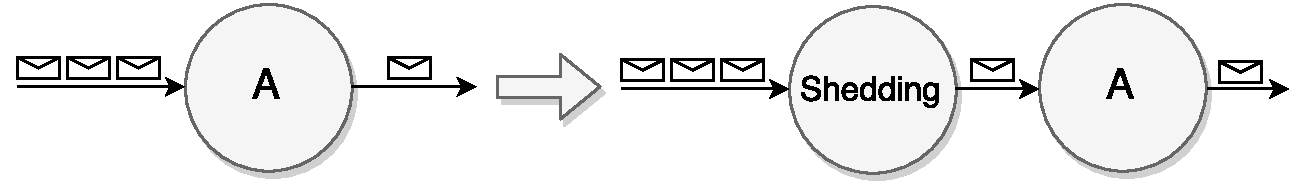
\includegraphics[scale=0.6]{images/LoadShedding.pdf}
	\caption{Load shedding en un SPS.}
	\label{fig:loadShedding}
\end{figure}

En el mundo de los SPS, varios poseen este tipo de estrategia, como por ejemplo S4 \citep{s4}, donde se establece una cota superior de eventos en cola, y en caso que su cola sea igual al l\'imite establecido, los eventos entrantes son descartados. Otro sistema que aplica esta t\'ecnica es Aurora \citep{aurora}, el cual se basa en procesamiento de datos por ventanas de tiempo, por lo que en caso de existir una ventana de tiempo con una mayor cantidad de eventos de lo estipulado, se descarta el exceso de eventos.

Si bien esta t\'ecnica \normalsize{posee un bajo c\'omputo computacional}, siendo pensada para la disminuci\'on r\'apida de carga, se introduce al sistema una baja en la precisi\'on y fiabilidad en los resultados. Por ejemplo, en el caso de la transferencia de video no es trascendental, dado que son pocos los pixeles perdidos, pero en una recopilaci\'on y an\'alisis de estad\'isticas, esto da una menor precisi\'on de la informaci\'on obtenida por el sistema, dado que puede perderse informaci\'on que est\'e relacionada con los comportamientos estudiados.

\subsection{Migraci\'on}
\label{sec:migracionBC}
%Tambi\'en se encuentra la migraci\'on, en el cual seg\'un el estado del sistema se migran los operadores de un nodo a otro. En \citep{XingZH05} se implementa   esta t\'ecnica, y si bien genera una menor carga en distintos nodos, produce un alto costo en la transferencia de los datos. Al realizar la transferencia de los datos, existe una menor tolerancia a fallos, a ra\'iz de lo cual, se propone el uso de un b\'uffer en el sistema, aumentando sus costos \citep{PittauACA07}.

La t\'ecnica de migraci\'on est\'a basada en el traspaso de un operador de un nodo a otro, seg\'un el estado del sistema. En la Figura \ref{fig:migracion} se puede apreciar dos nodos, los cuales poseen tres y dos operadores respectivamente, pero debido a una sobrecarga del nodo 1 se realiza una migraci\'on del un operador al nodo 2, ya que \normalsize{\'este \'ultimo} se encuentra con menor carga. De esta manera, se reparten homog\'eneamente la carga.

Si bien no existe una implementaci\'on que utilice la perspectiva seg\'un los recursos l\'ogicos, si existe una que utiliza la perspectiva seg\'un los recursos f\'isicos como es el caso de Borealis, el cual fue explicado anteriormente \citep{XingZH05}. Una de las principales cr\'iticas que se realiza a esta t\'ecnica, es que puede existir una falla en la comunicaci\'on del operador, donde no existe un mecanismo para evitar la p\'erdida de los datos. Debido a lo anterior, es que se propone el uso de \textit{buffer}, el cual respalde la informaci\'on, aumentando los costos del sistema \citep{PittauACA07}.

\begin{figure}[!ht]
	\centering
	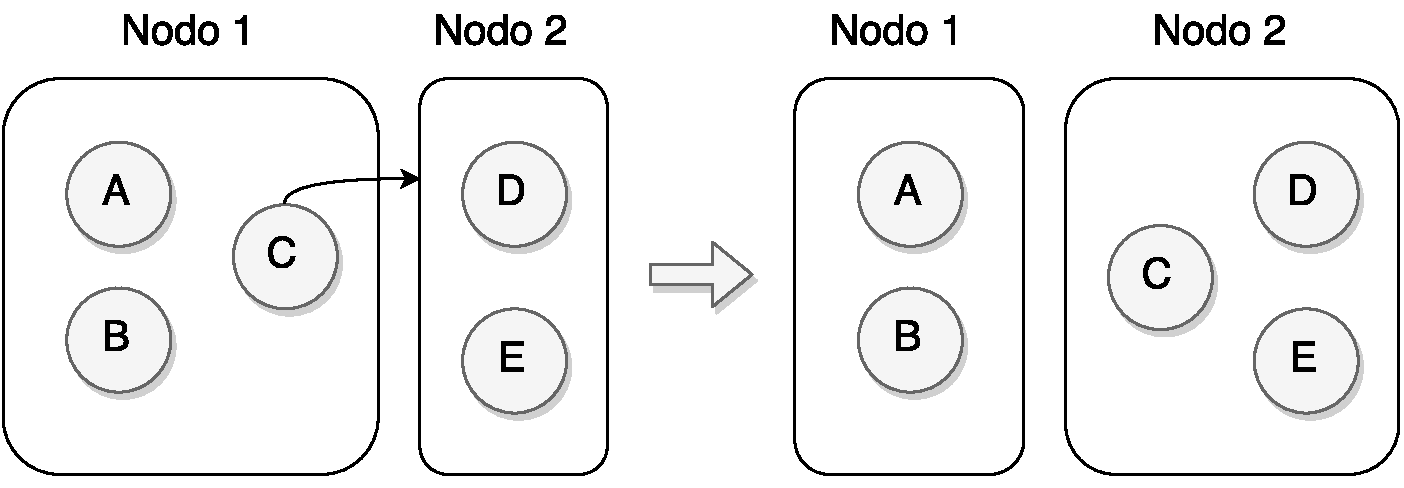
\includegraphics[scale=0.45]{images/Migracion.pdf}
	\caption{T\'ecnica de migraci\'on en un SPS.}
	\label{fig:migracion}
\end{figure}

\subsection{Fisi\'on}
\label{sec:fisionBC}

%Desde otra perspectiva, existen las t\'ecnicas de paralelizaci\'on y replicaci\'on, las cuales se utilizan en caso de sobrepasar un umbral, el cual depende de la carga de un operador, nodo, entre otras variables. El primero consiste en paralelizar una tarea, la cual est\'a determinada por un conjunto de operadores, en otro nodo f\'isico \citep{IshiiS11}. En cambio, la replicaci\'on consiste en replicar un operador a nivel l\'ogico del grafo \citep{MadsenTZ14}. Una de las caracter\'isticas que existen en este tipo de soluciones es la elasticidad, que consiste en la capacidad de aumentar o disminuir la cantidad de operadores seg\'un la necesidad del sistema.

Otra t\'ecnica utilizada en el balance de carga es la fisi\'on, o tambi\'en llamada replicaci\'on, que permite paralelizar el procesamiento, la cual consiste en crear una r\'eplica paralela del operador, sin perder el funcionamiento y estado. En Figura \ref{fig:fision} se presenta un operador A, el cual en primera instancia recibe un flujo de entrada $q_1$ y genera un flujo de salida $q_2$. Sin embargo, dado que este operador se sobrecarga, se procede a replicar, por lo que se hace necesario dos operadores auxiliares, \normalsize{en caso de ser un operador con estado} \citep{WuKWO12}, los cuales son el operador \textit{Split} y \textit{Merge}. Estas fases son necesarias para distribuir y juntar la informaci\'on respectivamente, y en general son de bajo costo. En caso de ser necesario replicar el operador \textit{Merge}, debe existir un \textit{merge} de las distintas r\'eplicas de \'este, lo cual hace m\'as complejo el dise\~no del sistema, por lo que se omite su replicaci\'on.

En algunos SPS el \textit{split} y el \textit{merge} son operadores que deben ser realizados por el programador, y no de forma autom\'atica por el sistema, como S4 o Storm. Una de las caracter\'isticas que se posee de esta t\'ecnica es que permite generar un sistema el\'astico, donde se puede aumentar o disminuir la cantidad de operadores seg\'un los requerimientos del sistema.

\begin{figure}[!ht]
	\centering
	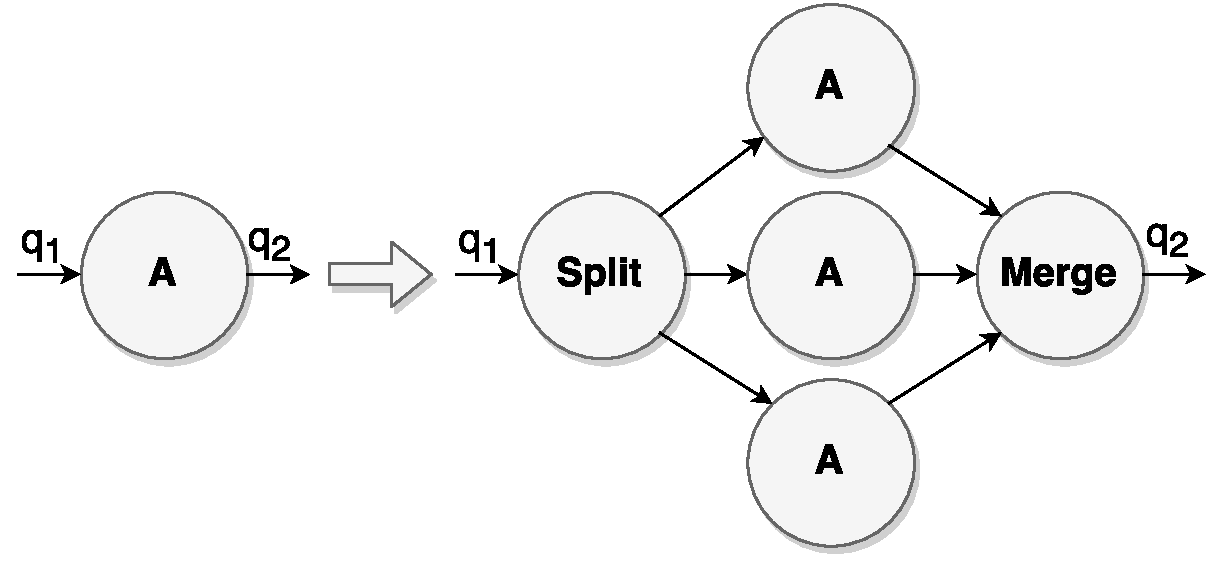
\includegraphics[scale=0.4]{images/Fision.pdf}
	\caption{T\'ecnica de fisi\'on en un SPS.}
	\label{fig:fision}
\end{figure}

%Una aplicaci\'on de la t\'ecnica de paralelizaci\'on seg\'un el enfoque est\'atico, es la paralelizaci\'on de tareas de Storm \citep{stormtwitterdoc}, donde un conjunto de operadores realizan una tarea, indicado la cantidad de tareas que se desean ejecutar paralelamente en el sistema.

%Un ejemplo aplicado de esta t\'ecnica seg\'un el enfoque dińamico es StreamCloud \citep{GulisanoJPSV12}, que dada la cantidad de consultas que van llegando al sistema, se paralelizan las tareas existentes. Uno de los problemas que surge en estos casos son las operaciones con estado, como lo son los contadores o algoritmos de orden. La soluci\'on planteada es poseer un operador que realiza la tarea de \textit{merge}, que consiste en recibir las salidas de las tareas paralelas, agrupando los datos y proporcionando una salida seg\'un lo realizado por cada uno de las operaciones \citep{GedikSHW14}.

Una aplicaci\'on que utiliza la t\'ecnica de fisi\'on bajo el enfoque est\'atico, es la paralelizaci\'on de tareas de Storm \citep{bookstorm}. Aqu\'i se debe indicar en la topolog\'ia del grafo la cantidad de operadores necesarios para realizar una tarea. De esta manera, por cada tarea se asigna un proceso, el cual tiene a su disposici\'on $n$ hebras seg\'un la cantidad de operadores que se desea para cumplir dicha tarea.

Otro sistema que utiliza esta t\'ecnica, bajo un enfoque din\'amico, es \textit{StreamCloud} \citep{GulisanoJPSV12}. Seg\'un la cantidad de consultas realizadas al sistema se aumenta o disminuye la cantidad de operadores que cumplen las tareas que se solicitan. Para esto, es necesario un operador que distribuya los datos, denominado \textit{split}, y uno que junte la informaci\'on entregadas por las r\'eplicas del operador, denominado \textit{merge}. \normalsize{Por lo que} este sistema s\'olo soporta ciertas operaciones, de tal manera que se creen de forma autom\'atica los operadores de \textit{split} y \textit{merge}. De esta manera, no existe problemas con los operadores con estado, como lo son los contadores y algoritmos de ordenamiento, dado que autom\'aticamente realiza el procedimiento de separaci\'on y uni\'on de los datos. Una de las caracter\'isticas principales de este sistema, es que aplica el concepto de elasticidad, que aumenta y disminuye la cantidad de operadores seg\'un lo requerido por el sistema.

Otros trabajos como \citep{GedikSHW14, SchneiderAGBW09} tambi\'en aplican este m\'etodo, y paralelizan las tareas de forma el\'astica, y con par\'ametros similares, s\'olo que su implementaci\'on es distinta, debido que \'este propone utilizar \textit{Cloud} para el uso del SPS. De esta manera, el enfoque se basa en la paralelizaci\'on de las tareas entre las distintas m\'aquinas.

En \citep{FernandezMKP13}, aplican fisi\'on en el caso que exista un cuello de botella en un operador. Para la detecci\'on de estas situaciones, se posee un monitor, el cual est\'a consultando cada cierto per\'iodo de tiempo el estado de cada uno de los operadores. De esta manera, en caso que un operador sobrepase el umbral de carga establecido, el cual est\'a determinado por la utilizaci\'on de CPU se replique el operador. En la Figura \ref{fig:ejFision} se puede ver un sistema, en el cual el operador \textit{u} est\'a enviando un flujo de datos al operador \textit{o}. Una vez que \textit{o} se sobrecarga (cuello de botella),\normalsize{ \'este se replica tantas veces como sea necesario hasta reducir la carga hasta el umbral deseado.}

Dentro de las desventajas existentes por parte de estos trabajos realizados, es que no utilizan la historia del operador para analizar el comportamiento a futuro de la carga. El uso de sistemas de predicci\'on puede estabilizar el sistema cuando existen \textit{peaks} en el tr\'afico, debido que estos son detectados en el pasado, y se verifica si pueden ocurrir en el futuro. \normalsize{Otra} desventaja, es que en algunos trabajos es necesario detener la ejecuci\'on de la aplicaci\'on, cambiar el n\'umero de r\'eplicas y volver a iniciar, lo cual genera una p\'erdida de eventos.

\begin{figure}[!ht]
	\centering
	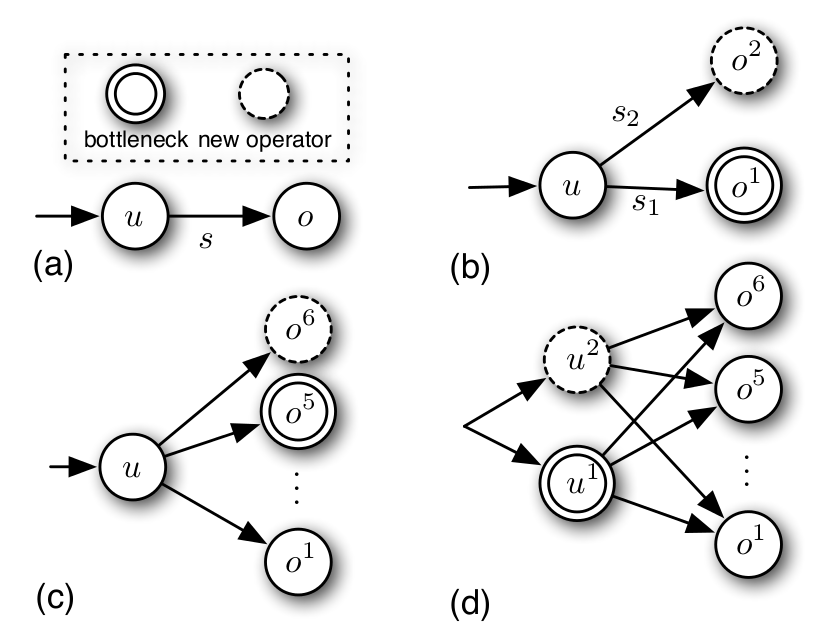
\includegraphics[scale=0.3]{images/EjFision.png}
	\caption{Ejemplo de replicaci\'on de los operadores \citep{FernandezMKP13}.}
	\label{fig:ejFision}
\end{figure}